% !Mode:: "TeX:UTF-8"
%% This is file `mcmthesis-demo.tex',
%% generated with the docstrip utility.
%%
%% The original source files were:
%%
%% mcmthesis.dtx  (with options: `demo')
%%
%% -----------------------------------
%%
%% This is a generated file.
%%
%% Copyright (C)

%% This work may be distributed and/or modified under the
%% conditions of the LaTeX Project Public License, either version 1.3
%% of this license or (at your option) any later version.
%% The latest version of this license is in
%%   http://www.latex-project.org/lppl.txt
%% and version 1.3 or later is part of all distributions of LaTeX
%% version 2005/12/01 or later.
%%
%% This work has the LPPL maintenance status `maintained'.
%%
%% The Current Maintainer of this work is Liam Huang.
%%
\documentclass{mcmthesis}
\mcmsetup{tcn = 43472, problem = E,
  sheet = true, titleinsheet = true, keywordsinsheet = false,
        titlepage = true, abstract = true}
\usepackage{palatino}
\usepackage{times}
 \usepackage{indentfirst}
\usepackage{lipsum}
\renewcommand{\sfdefault}{ptm}
\title{The Template for MCM Version }

\author{Team \# 43472}
\date{\today}


%\renewcommand\abstractname{Abstract}


\begin{document}
\begin{abstract}
Here SUMMARY start!

%\begin{keywords}
%keyword1; keyword2
%\end{keywords}
\end{abstract}

\maketitle

%tocloft texdoc tocloft
\tableofcontents

\newpage

\section{Introduction}
\subsection{Introduction}

	
	As the population increase drastically in last century, water scarcity has becoming a serious problem. This is not only because of the lack of the fresh water but also due to the inappropriate way to disposal waste water and refresh salt water. Social factors also have complex influence on water availability. There may be conflicts between water use for domestic, for industry, for agriculture and environmental protection. Taking account of the increasing grim situation of 
environment issue, water,which is an important part of whole ecosystem, should be seriously distributed. Hence, water scarcity is not only a geological problem, economic,ecological and social factors also should be considered about. 
	
	In order to avoid heading towards a thirsty earth, the International Clean water Movement (ICM) is interested in finding out the constraints on water supply. Therefore, following tasks are needed.

%These tasks are needed	

\begin{itemize}
\item minimizes the discomfort to the hands, or
\item maximizes the outgoing velocity of the ball.
\end{itemize}

	To be more specific, ICM want to investigate a single region. By using a general model we have designed, the analysis of the historical and current water use and the forecast of the water availability is requested.In order to accomplish these requirement, we should finish the mission listed bellow.

\begin{itemize}
\item the initial velocity and rotation of the ball,
\item the initial velocity and rotation of the bat,
\item the relative position and orientation of the bat and ball, and
\item the force over time that the hitter hands applies on the handle.
\end{itemize}




\begin{itemize}

\item the angular velocity of the bat,
\item the velocity of the ball, and
\item the position of impact along the bat.
\end{itemize}

\emph{center of percussion} [Brody 1986], \lipsum[5]



%=======
\begin{Theorem} \label{thm:latex}
\LaTeX
\end{Theorem}
\begin{Lemma} \label{thm:tex}
\TeX .
\end{Lemma}
\begin{proof}
The proof of theorem.
\end{proof}


\subsection{Fundamental Assumptions}

\section{Theory Methodology}
\subsection{Artificial Neural Network}

The artificial neural network is the complex network composed by numerous simple nerve cells to simulate the thinking process of human brain. There is no need of any explicit math model in neural network, but only enough training data for it to "learn" the complex nonlinear relationship. Compared to traditional prediction method, the artificial neural network(ANN) works through self-learning, self-adaption and presents good quality of fault-tolerant in pattern-recognition. We will apply this method during our modeling. 

There are many learning algorithms of neural network. We will use Error Back Propagation(BP) algorithm\textbf{[]}. The structure consists of input layer, output layer and several hidden layers.

The BP algorithm has two main phase: a feed forward phase in which the external input information at the input nodes is propagated forward to compute the output information signal at the output unit, and a backward phase in which modifications to the connection strengths are made based on the differences between the computed and observed information signals at the output units. 

Assume that there are $m$ layers in the network and $y_{i}^{m}$ represents the output of the $jth$ node in the $mth$ layer. $y_{j}^{0}$ equals to $x_{j}$,i.e.,the $jth$ input node.$W_{ij}^{m}$ represents the connected weight from $y_{j}^{m-1}$ to $y_{j}^{m}$. $\theta_{j}^{m}$ represents the threshold of the $jth$ node in the $mth$ layer. We train the BP network by these steps.
\begin{enumerate}[i]
\item Assign each weight and threshold with a random value from the range $(-1,1)$.
\item Choose one data pair $(x^{k},T^{k})$ from the training data set and assign the input variable to input layer($m=0$), all nodes in this layer follow the equation$$y_{i}^{0}=x_{i}^{k} $$ $k$ represents the num. of training graph.
\item Signals propagate forward by the network, i.e. according to the equation$$y_{j}^{m}=F(s_{j}^{m})=F(\sum_{i} W_{ij}^{m}y_{j}^{m-1}+\theta_{j}^{m} )$$Compute the output $y_{j}^{m}$ of each node $j$ from the first layer to the end. $F(s)$ is the Sigmoid Function.
\item Compute the error of each node in output layer:$$\delta_{j}^{m}=y_{j}^{m}=(1-y_{j}^{m})(T_{j}^{k}-y_{j}^{m})$$ The error comes from the differences between real outputs and goal values.
\item Compute the error of each node in previous layers:$$\delta_{j}^{m}=F^{'}(s_{j}^{m-1}\sum_{i} W_{ij}^{m}\delta_{i}^{m})$$ It depends on propagating error backward layer by layer.
\item Modify weights and thresholds backward layer by layer:
$$W_{ij}^{m}(t+1)=W_{ij}^{m}(t)+\eta \delta_{j}^{m}y_{i}^{m-1}+\alpha \Big[W_{ij}^{m}(t)-W_{ij}^{m}(t-1) \Big]$$
$$\theta_{j}^{m}(t+1)=\theta_{j}^{m}(t)\eta\delta_{j}^{m}+\alpha\Big[\theta_{j}^{m}(t)-\theta_{j}^{m}(t-1) \Big]$$
In the equations, t mis iterations count;$\eta$ is the learning speed[$\eta \in (0,1)$];$\alpha$ is dynamic coefficient [$\alpha \in (0,1)$]
\item run to ii and turn into next graph, repeat steps ii~vii until network global error$$E=\sum_{k}\sum_{j}(T_{j}^{k}-y_{j}^{m})^{2}/2$$satisfies with the preset precision. 
\end{enumerate}
After neural network having been trained and we got appropriate weights and thresholds. Then it can be used to predict and analysis.

\section{The Models}
We construct the evaluation model based on the Water Stress Indictor(WSI) which is mentioned by Vladimir Smakhtin, Carmen Revenga and Petra D{\"o} ll[].It is simple and used in many world environment report. We use Water Capacity Index(WCI) to measure the ability of providing fresh water. If the WCI is high, it means that renewable water is much more than water demand of human and the whole ecosystem can maintain a better condition. We need another two model to calculate two variables used for calculating WSI,i.e.Natural Renewable Water Supply Model and Water Demand Model.
 
The water supply and demand model is based on the analysis of both natural and human factors, as well as their interrelationship. We shall give the model of natural renewable water supply and actual demand of corresponding population. And finally a method would be presented to measure the ability of a region to provide clean water to meet the need of its population. 
\subsection{WCI Measurement Model}
\subsubsection{Calculation}
We define WCI as $$WCI=\frac{Renewable\quad Water\quad Supply}{Water\quad Demand}$$
There are two key variables in this equation.
\begin{itemize}
\item
\textbf{Water Demand}:  It is equal to water withdrawal.We can calculate by various factors in out Water Demand model.
\item \textbf{Renewable Water Supply}:  We consider renewable water source as we evaluate the ability for sustainable development. We only take the he long-term mean annual runoff (MAR) to represent renewable water supply because other manual factors such as wastewater disposal and sea water desalination can be the negative factors in water demand. There os also another model for MAR own.
\end{itemize}

\subsubsection{Evaluation Standard}
We define the standard as below.The standard seems arbitrary while it comes from experience of statistics data.\textbf{[]}.
\begin{itemize}
\item $WCI>4$, the water resource is rich.
\item $1.5<WCI<4$, the water is moderately stress and ecosystem has the possibility to deteriorate.
\item $WCI<1.5$, the water withdrawal is overloaded and it should take actions to improve the conditions immediately.
\end{itemize}
 We choose such standard dependent on two fact:
 \begin{itemize}
\item The environment requires enough water to maintain the ecosystem,i.e.Environmental Water Requirements (EWR).For each river, EWR is almost the same percent of the MAR and it is no more than 50\% commonly. 
\item MAR will change in different seasons and we must consider the minimum discharge in some month and ensure fresh water use in extreme conditions.

\end{itemize}
\subsection{Natural Renewable Water Supply Model}
\subsubsection{Natural Renewable Water Supply}

The quantity of natural renewable water that could be used by human is mainly influenced by the runoff of watershed of the region. The runoff of watershed incorporates all surface water, ground water and any natural sources that can be reused. All of them have complex and subtle relationship with each other, so we just consider them as a whole, i.e., a dynamic criteria. The runoff of the watershed is determined by numerous factors which are interconnected. These factors have more explicit natural regulations than just the runoff of watershed itself. While making prediction, we choose these factors as variables. And we choose the principle as following: 

While there exist numerous such predictive variables, many of these variables are interconnected and not well understood; a model that incorporates dozens of such variables would only offer slight improvements in accuracy than one that incorporates a few inherently different variables, and would be much more difficult to interpret.

The variables chosen are precipitation, temperature, basin area and vegetation coverage degree. The relationship between these factors and runoff of watershed is very complex to illustrated by any liner model, so we build a neural network of three layers, as shown in figure 1. The data of the past of the region are used for training. 
%LaTeX插图指南
\begin{figure}[h]
	\small
	\centering
	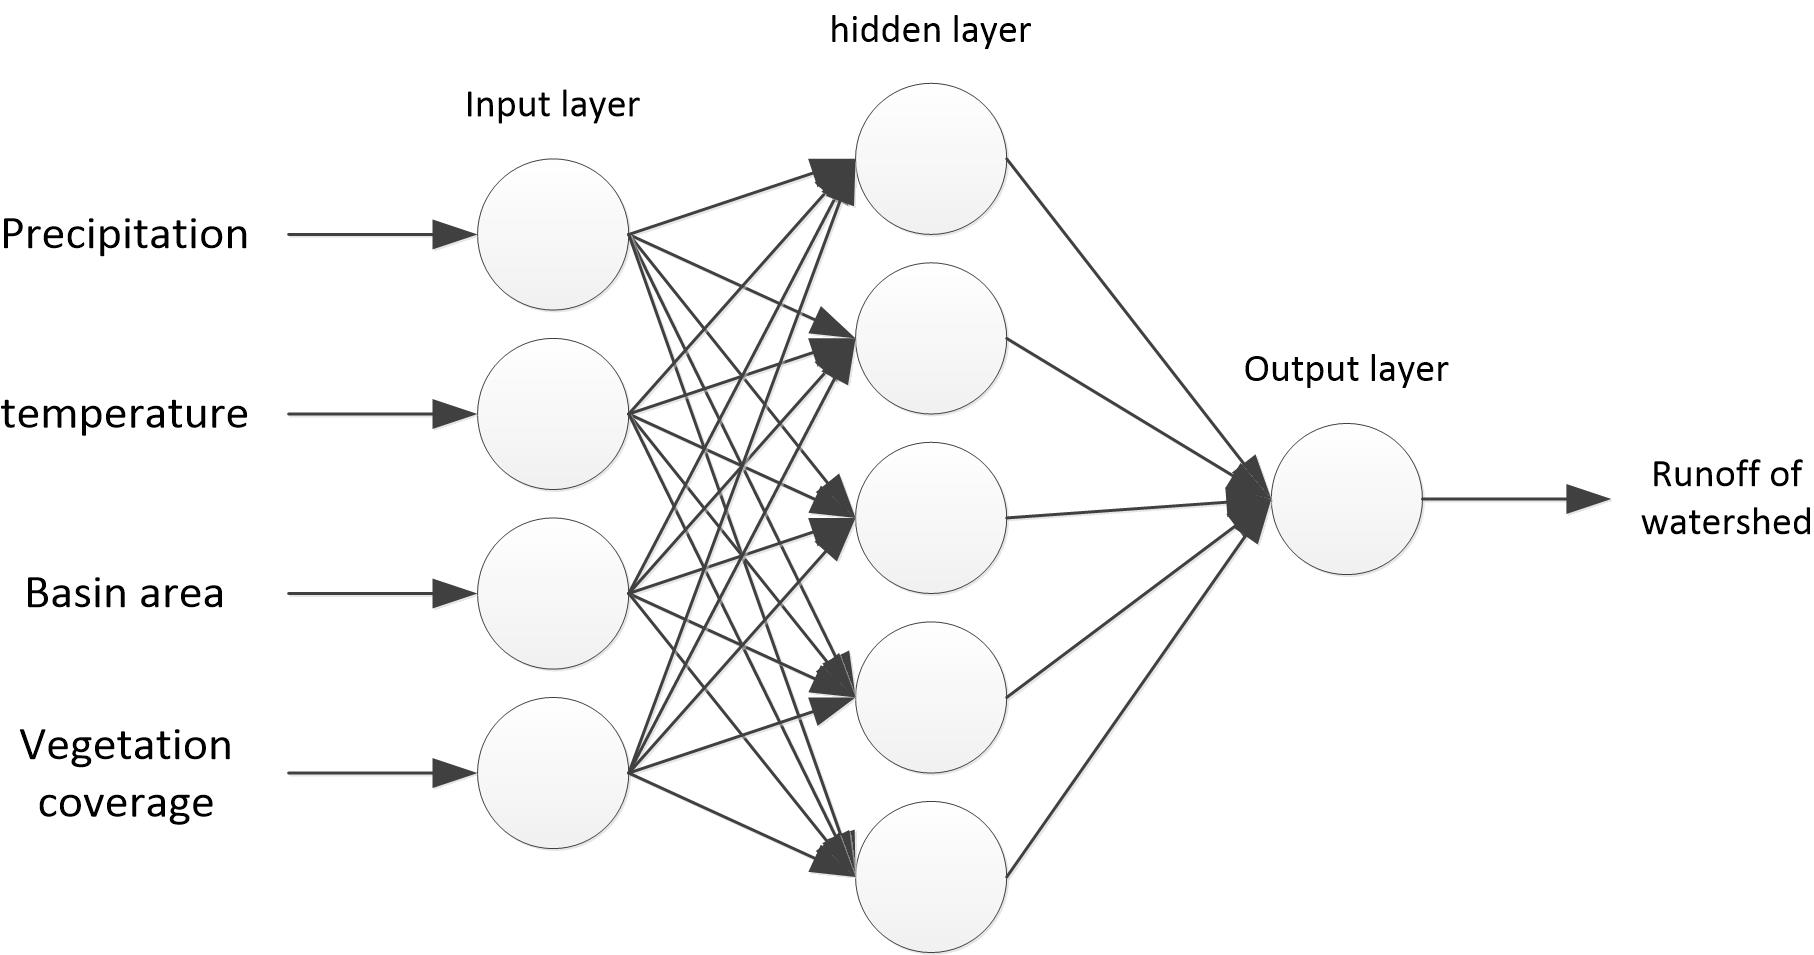
\includegraphics[width=10cm]{neural.jpg}
	\caption{Neural network in Natural Renewable Water Supply Model} \label{fig:Neural network in Natural Renewable Water Supply Model}
\end{figure}

%1,不要用子图,subfig,subfigure。
%2,尽量减少浮动环境,图尽量,缩小图的占位

\eqref{Neural network in Natural Renewable Water Supply Model}

After predicting the four factors, we input these factors to the input layer and get our prediction from the output layer. The overview of our natural renewable water supply model is shown in figure 2:

\begin{figure}[h]
	\small
	\centering
	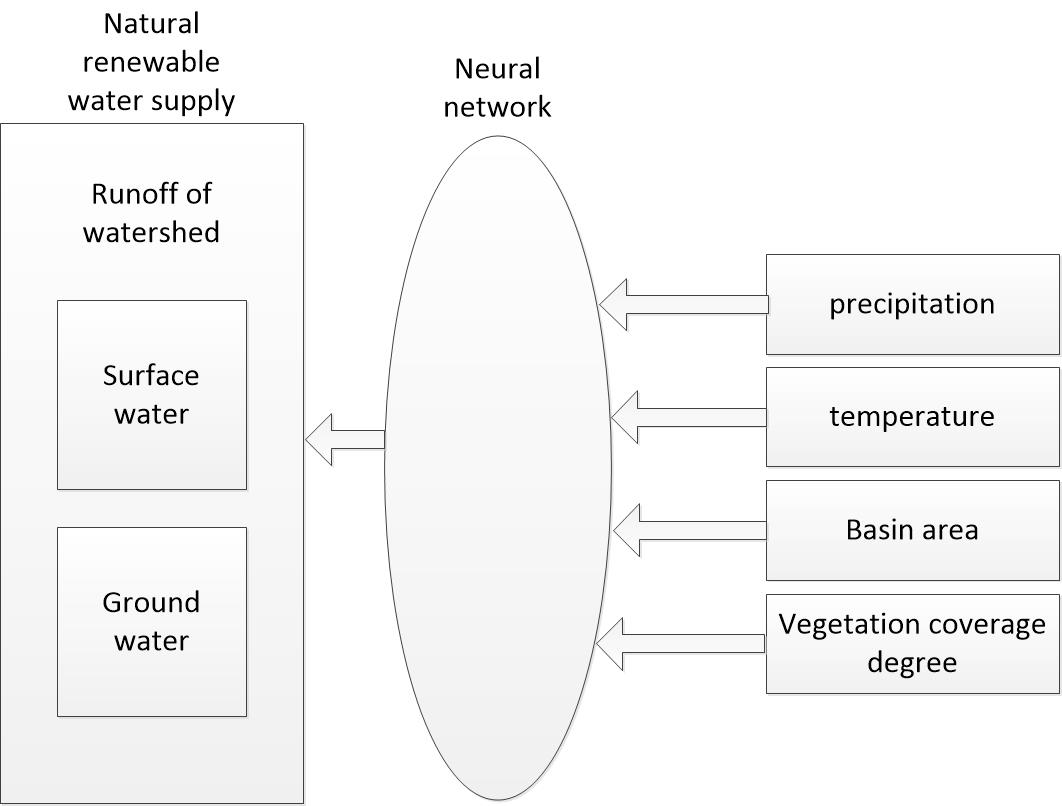
\includegraphics[width=10cm]{modelnatural.jpg}
	\caption{Factors flow in the model} \label{fig:bb}
\end{figure}


\subsubsection{Variable Prediction}
The variable chosen for prediction of runoff of watershed are precipitation, temperature, basin area and vegetation coverage degree. 

In short period of time, i.e., 15 years, the basin area actually changes very little. We consider it as constant. The vegetation coverage degree is mostly decided by human actions, i.e., government policy for vegetation coverage protection in one country. We should do the analysis when dealing with specific examples. 

Precipitation and temperature are not to predict as they are  
\subsection{Water Demand Model}
\subsubsection{Water Demand}
The actual consumption of water in a region can be illustrated through the water consumption of three levels of industry, personal consumption, and many other factitious factors. The sewage disposal and sea water desalination also replenish part of water consumption. They are determined mostly by the industrialization degree of the region.

We divided all these factors into industrial aspect, agriculture aspect and domestic aspect.
\begin{itemize}
\item Industrial aspect: water consumed for industrial use. 
\item Agriculture aspect: Water consumed for agriculture, i.e, irrigation, livestock, aquatic  products, etc. 
\item Domestic aspect: water consumed directly by its population for basic requirements of life. 

\end{itemize}

According to the principle of previous section, these three aspects consume water for inherently different means. Thus we could trace the regulation within each aspect and make prediction with relatively high accuracy. We should also consider the availability of historical data when choosing the predictive variables for each aspect.

For domestic aspect, the main consumer of domestic water is the general population. But they do not present an accurate linear relationship, as the water consumption is also determined by the standard of living. In highly-developed region, people tends to consume more water, but the distribution efficiency and water recycling rates would also increase. We take the assumption that this measure is correlated to standard of living, taken as the product of GDP/capita (as an approximation for spending power per person) and life expectancy. %%__注释[]

For industrial aspect, the total energy consumption was used, as industrial energy consumption is nearly linear to total energy consumption \textbf{[]} and is a rough measure of industrialization degree. Industrialization degree also depends on the degree of technological development. Highly developed industry would be more efficient with the use of water. Technological development was modeled as GDP/capita, in which higher GDP/capita would correspond to higher productivity per person enabled by more advanced technology.  %%__注释[]

For agricultural water use, we choose the agriculture land area and  precipitation. We assume that in a short period of time, i.e, the time duration we will analyze in the task of this ICM problem, the crop and livestock intensity in the farmland of a region does not change much, the quantity of aquatic products also remain constant. Under this assumption the water required for agricultural purpose presents a linear relationship with the land area of farmlands. The natural rain complements the consumption for irrigation, we should also count it in.

In summary, we choose the following six factors to make prediction:

\begin{itemize}
\item Total energy consumption
\item Population
\item Gross Domestic Product
\item Life expectancy estimates
\item Precipitation
\item Temperature
\end{itemize}

For economic aspect, Total energy consumption and GDP both reflects the industrialization degree. For natural aspect, agriculture land area and precipitation determine the water consumption for agriculture. For factitious aspect, population life expectancy determine the domestic water consumption. 


After predicting these factors, we input them into neural network that has been trained by previous data and get our prediction of water demand. The overview of this model is shown in figure 3:

\begin{figure}[h]
	\small
	\centering
	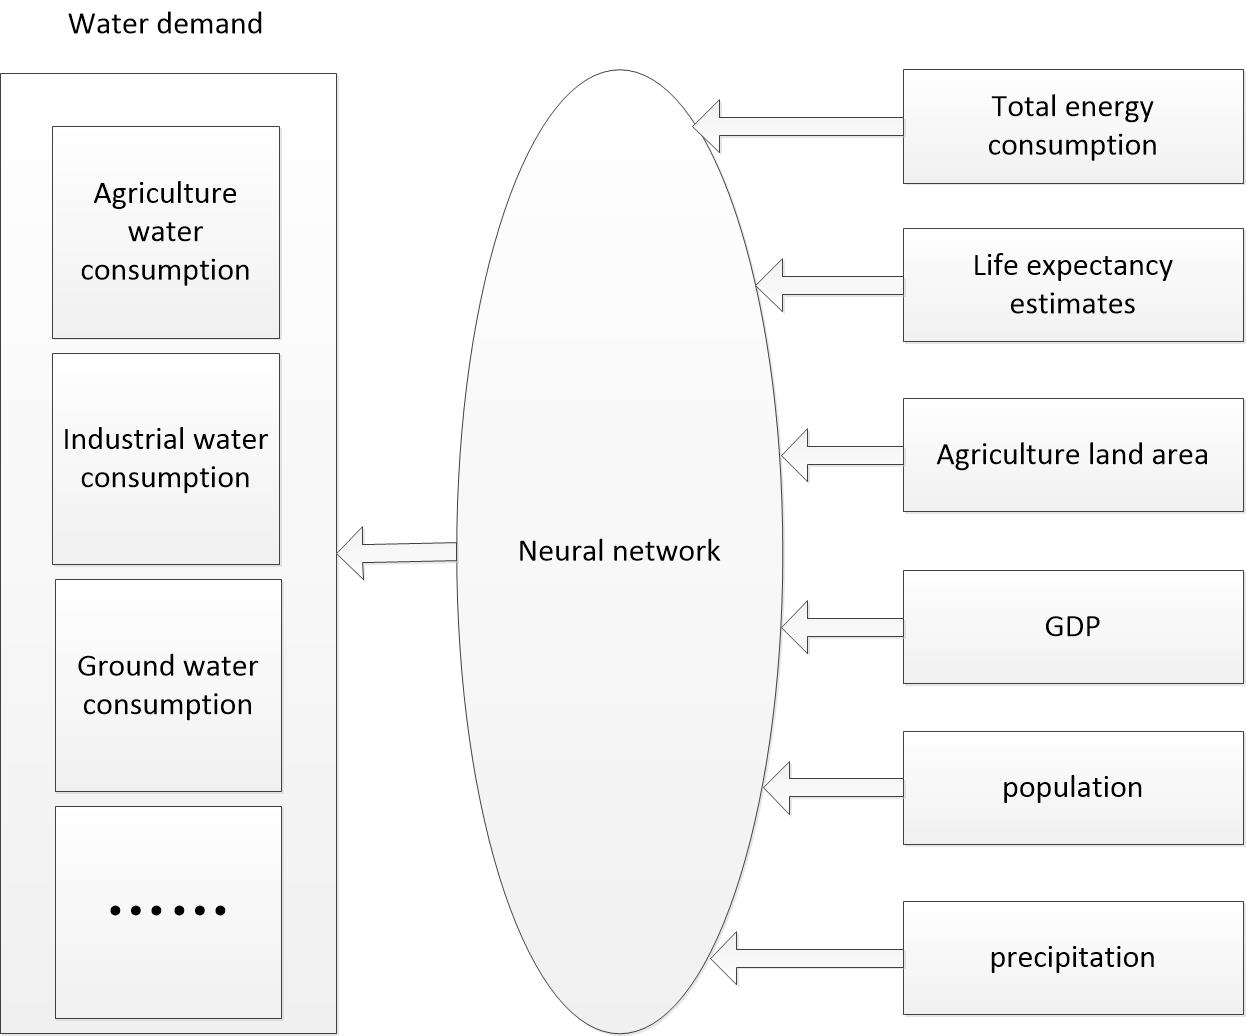
\includegraphics[width=10cm]{waterdemand.jpg}
	\caption{Factors flow in the Water Demand model} \label{fig:cc}
\end{figure}

\subsubsection{Variable Prediction}

\subsection{model summary and criteria for water scarcity}
The overview of our whole model of water supply and demand is represented in figure 3:
\begin{figure}[h]
	\small
	\centering
	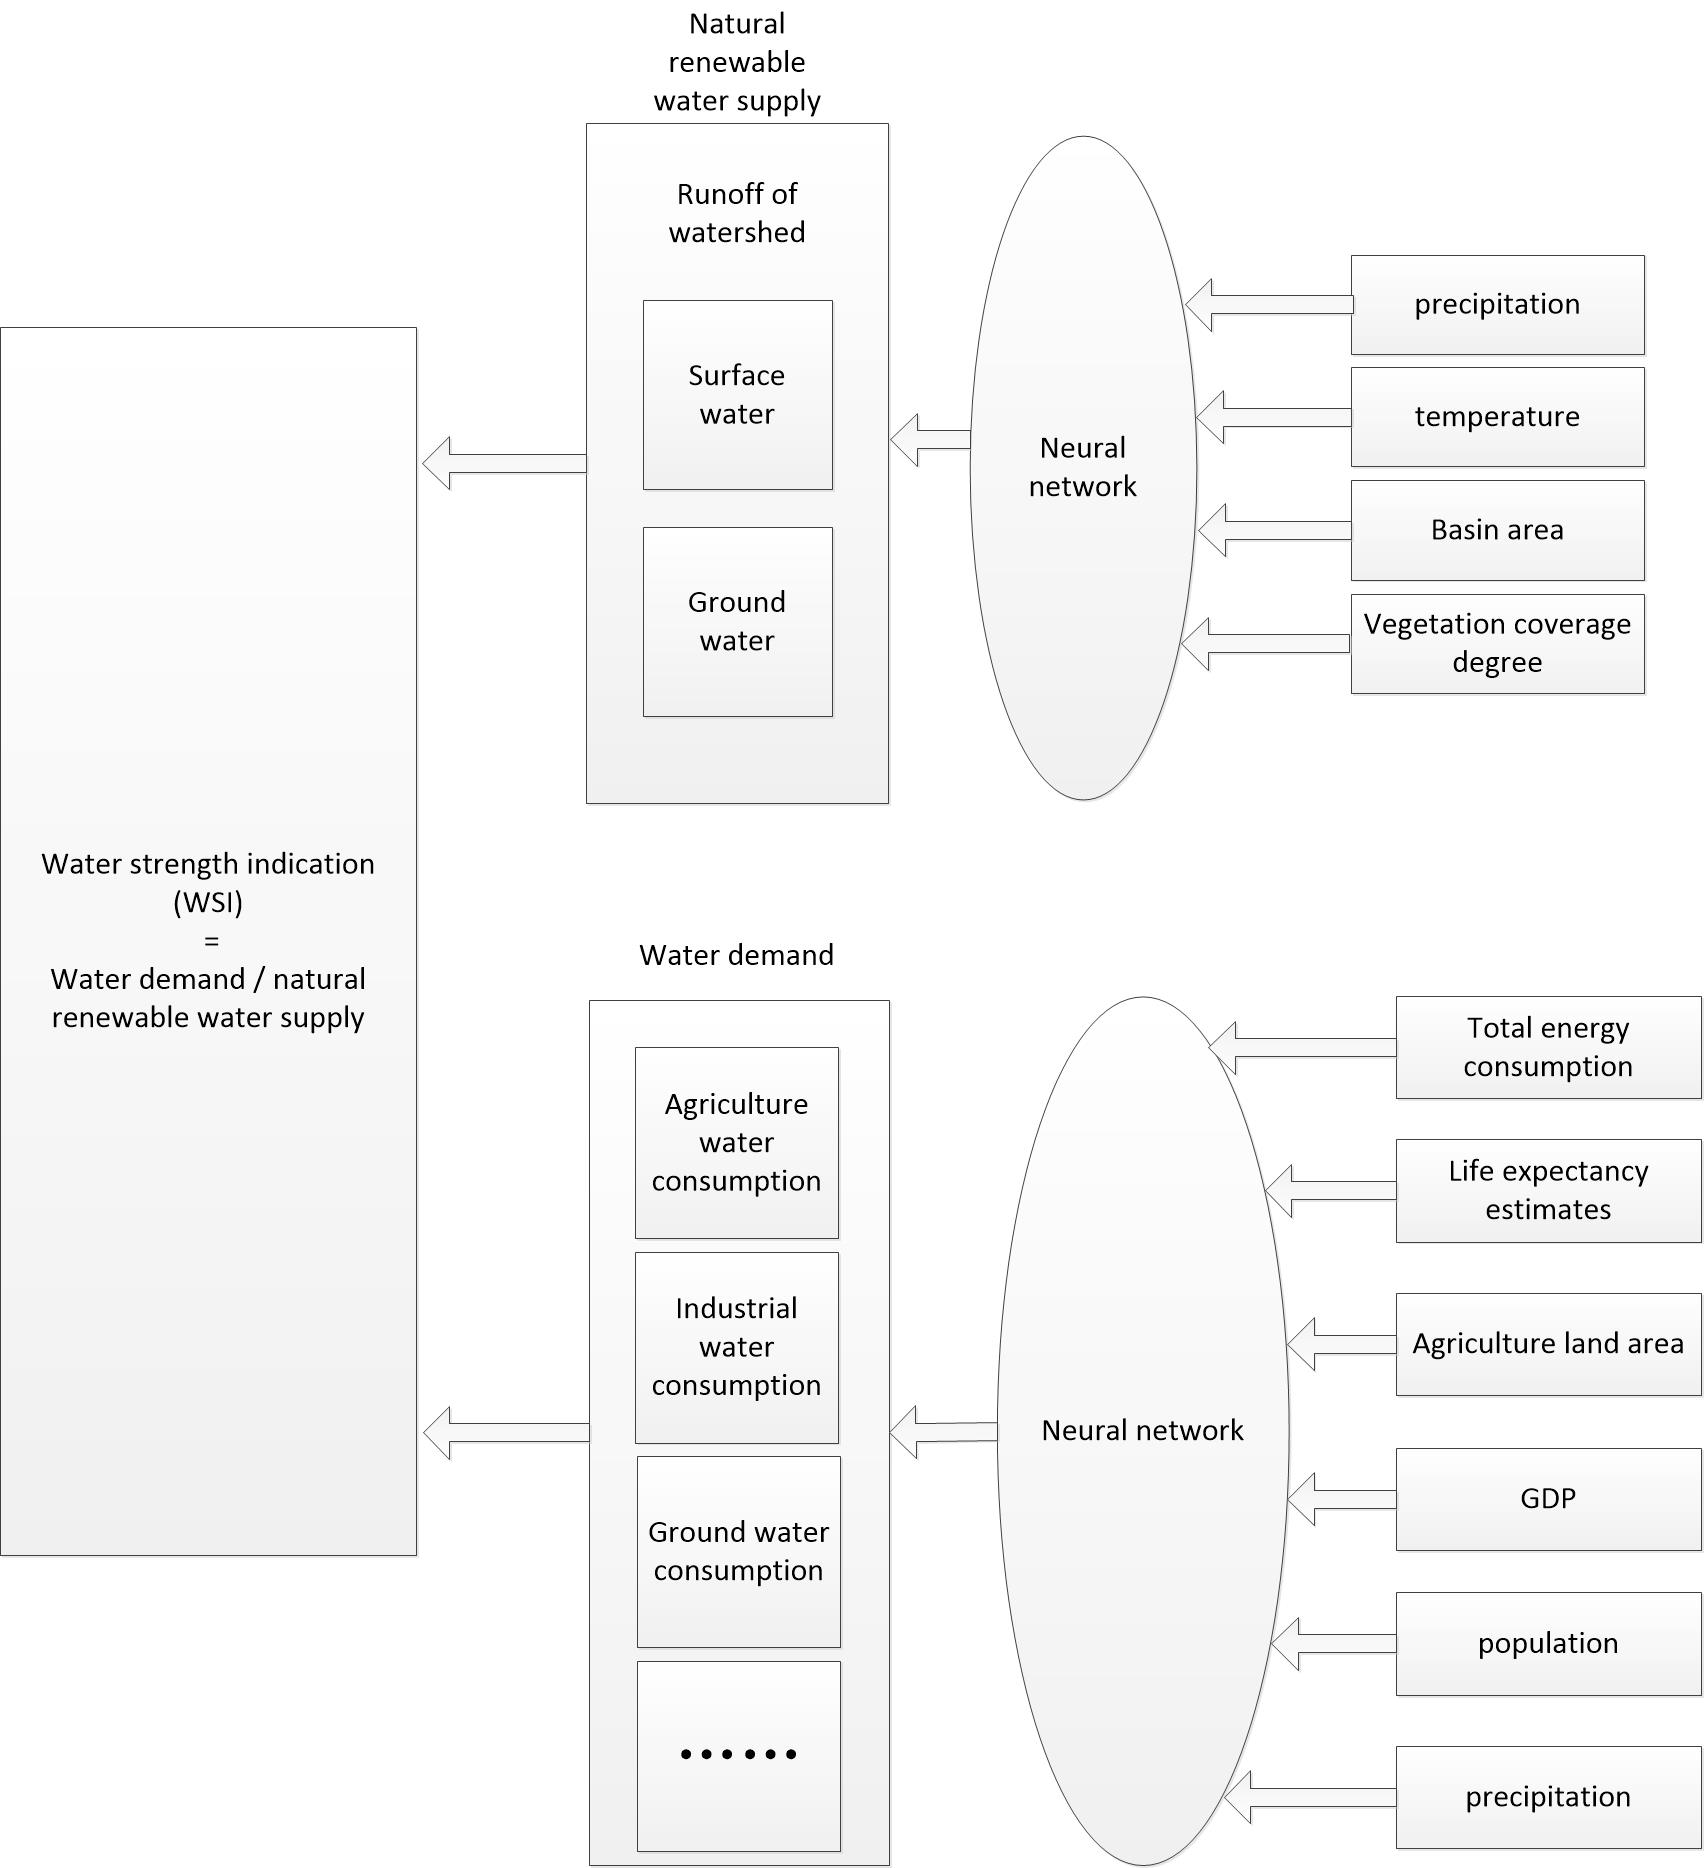
\includegraphics[width=10cm]{model.jpg}
	\caption{Whole model to measure the ability of providing water sustainablely} \label{fig:dd}
\end{figure}

\section{Analysis of water availability in specific region}

\subsection{Historical and current situation}
	The situation of water source is various from area to area, from season to season.In this section, we would like to take      \textbf{Germany}for example.
\section{The Model Results}


\section{Validating the Model}


\section{Conclusions}


\section{A Summary}


\section{Evaluate of the Mode}

\section{Strengths and weaknesses}


\subsection{Strengths}
\begin{itemize}
\item \textbf{Applies widely}\\
This  system can be used for many types of airplanes, and it also
solves the interference during  the procedure of the boarding
airplane,as described above we can get to the  optimization
boarding time.We also know that all the service is automate.
\item \textbf{Improve the quality of the airport service}\\
Balancing the cost of the cost and the benefit, it will bring in
more convenient  for airport and passengers.It also saves many
human resources for the airline. 
\end{itemize}

%(author, 1998)  APA style.

\begin{thebibliography}{99}
\bibitem{1} D.~E. KNUTH   The \TeX{}book  the American
Mathematical Society and Addison-Wesley
Publishing Company , 1984-1986.
\bibitem{2}Lamport, Leslie,  \LaTeX{}: `` A Document Preparation System '',
Addison-Wesley Publishing Company, 1986.
\bibitem{3}\url{http://www.latexstudio.net/}
\bibitem{4}\url{http://www.chinatex.org/}
\end{thebibliography}

%\hspace{2em}

\end{document}

%%
%% This work consists of these files mcmthesis.dtx,
%%                                   figures/ and
%%                                   code/,
%% and the derived files             mcmthesis.cls,
%%                                   mcmthesis-demo.tex,
%%                                   README,
%%                                   LICENSE,
%%                                   mcmthesis.pdf and
%%                                   mcmthesis-demo.pdf.
%%
%% End of file `mcmthesis-demo.tex'.
